\documentclass[a4paper, 11pt, chapterprefix=false]{report}

\usepackage[top=3cm, bottom=2.5cm, left=2.5cm, right=2.5cm]{geometry}
\usepackage{amsmath, amssymb, amsthm}
\usepackage{setspace}
\usepackage{graphicx}
\usepackage{enumitem}
\usepackage{kotex}
\usepackage{hyperref}
\usepackage{xcolor}
\usepackage{url}
\usepackage{listings}
\usepackage{courier}
\usepackage[htt]{hyphenat}
\usepackage{biblatex}

\usepackage{titlesec, blindtext, color}
\usepackage{lipsum}
\usepackage{indentfirst}

% Referencing Style
\let\OLDthebibliography\thebibliography
\renewcommand\thebibliography[1]{
  \OLDthebibliography{#1}
  \setlength{\parskip}{0pt}
  \setlength{\itemsep}{0pt plus 0.3ex}
}

\addbibresource{references.bib}

%\renewcommand{\thechapter}{제 \arabic{chapter} 장}
\renewcommand{\thesection}{\arabic{section}}
\renewcommand{\contentsname}{목차}

\newtheorem{theorem}{Theorem}

\newcommand{\ud}{\underline}
\renewcommand{\vec}{\mathbf}
\newcommand{\htimes}{\ud{\times}}
\newcommand{\hplus}{\ud{+}}
\newcommand{\hrotate}{\ud{rotate}}
\newcommand{\alert}[1]{\textcolor{red}{#1}}

\setlist[itemize]{noitemsep}
\setlist[enumerate]{noitemsep}
\setstretch{1.7}

\definecolor{gray75}{gray}{0.75}
\titleformat{\chapter}[hang]
  {\LARGE\bfseries\center}{제 \thechapter{ 장}\quad}{0pt}{}
\titleformat{\section}[hang]
  {\Large\bfseries}{제 \thesection{ 절}\quad}{0pt}{}
\titlespacing{\chapter}{0pt}{-40pt}{40pt}

\begin{document}

\chapter*{요약}
\begin{quote}
동형암호 기반 안전한 딥러닝 추론 시스템은 학술계 및 산업계에서 급히 떠오르고
있는 주제이다. 뉴럴 네트워크의 추론 과정을 수행함과 동시에 완벽한 사용자
개인정보 보호를 달성할 수 있기 때문이다. 많은 연구 주제에서 딥러닝에 사용되는
컴포넌트를 동형암호의 단위 연산으로 분해하여 구현하거나, 그것을 고/저수준
단계에서 최적화시키는 일을 활발히 진행하고 있다. 하지만 이 과정이 마무리된 이후,
동형암호의 특성에 맞도록 모델을 학습하고 세부 조정하여 성능(정확도)을 유지하는
논의도 필요할 것이다. 본 연구에서는 동형암호 체계 상에서 딥러닝 네트워크 추론
과정을 시뮬레이션하고, 정확도를 최대한 보존하는 모델 구성 방법을 찾는 것을
목표로 한다. 암호문으로부터 계산할 수 없는 분기문(conditional instruction)을
근사다항식으로 대체하고, 그 과정에서 발생하는 정확도 하락을 최소화하는 모델 학습
방법론을 시뮬레이션을 통해 실험적으로 밝혀낸다. 이로부터 암호화된 사용자
데이터를 복호화 과정 없이 계산하는 안전한 딥러닝 추론 시스템의 상용 가능성을
재고한다.
\end{quote}

\begin{center}
  \textbf{주요어: 동형암호, 안전한 딥러닝 추론, 시뮬레이션, 근사다항식, 모델 학습}
\end{center}

\tableofcontents

\chapter{서론}

\section{연구 동기 및 목표}

동형암호 기반 안전한 딥러닝 추론 시스템은 학술계 및 산업계에서 급히 떠오르고
있는 주제이다. 뉴럴 네트워크의 추론 과정을 수행함과 동시에 완벽한 사용자
개인정보 보호를 달성할 수 있기 때문이다. 많은 연구 주제에서 딥러닝에 사용되는
컴포넌트를 동형암호의 단위 연산으로 분해하여 구현하거나, 그것을 고/저수준
단계에서 최적화시키는 일을 활발히 진행하고 있다. 하지만 이 과정이 마무리된 이후,
동형암호의 특성에 맞도록 모델을 학습하고 세부 조정하여 성능(정확도)을 유지하는
논의도 필요할 것이다.

본 연구에서는 동형암호 체계 상에서 딥러닝 네트워크 추론 과정을 시뮬레이션하고,
정확도를 최대한 보존하는 모델 구성 방법을 찾는 것을 목표로 한다. 암호문으로부터
계산할 수 없는 분기문(conditional instruction)을 근사다항식으로 대체하고, 그
과정에서 발생하는 정확도 하락을 최소화하는 모델 학습 방법론을 시뮬레이션을 통해
실험적으로 밝혀낸다. 이로부터 암호화된 사용자 데이터를 복호화 과정 없이 계산하는
안전한 딥러닝 추론 시스템의 상용 가능성을 재고한다.

\section{동형암호}

동형암호(Homomorphic Encryption)는 복호화 과정 없이 암호화된 데이터만으로 연산할
수 있는 체계이다. 암호문으로부터 특정한 연산이나 함수를 수행한 결과는 또 다른
암호문이 되며, 이를 복호화한 결과는 평문에서 동일한 연산이나 함수를 계산한 것과
일치한다.

이러한 특성 덕분에 동형암호를 이용하면 개인정보의 유출 없이 여러 유의미한 계산을
수행할 수 있다. 예를 들어, 서울대학교 학생들의 학점을 암호화한 데이터가 주어질
때 그들의 평균과 분산을 계산해야하는 상황을 고려하자. 고전 암호체계에서는
암호문만으로 유의미한 연산을 전혀 수행할 수 없으므로, 계산을 위해 원점수가
노출될 위험이 있는 평문으로 복호화시키는 과정이 필수적이다. 하지만 동형암호를
사용하면 이러한 위험 부담 없이 암호화된 상태에서 덧셈과 곱셈 연산으로 통계치를
획득할 수 있다. 이렇듯 동형암호는 안전한 통계량 계산, 비밀 투표, 그리고 딥러닝
추론 등 다양한 응용 가능성을 내재하고 있다.

\section{혜안 (HEaaN)}

혜안(HEaaN)은 부동소수점 기반의 대표적인 동형암호 구현체이다. \cite{heaan2017}
마치 크기가 고정된 1차원 텐서처럼 실수(real number) 데이터를 벡터화시켜 저장하고
연산을 수행한다.  지원하는 연산은 덧셈($+$), 곱셈($\times$), 그리고
회전($rotate$)이 있다.
\begin{gather*}
    (a_1, a_2, \dots, a_n) + (b_1, b_2, \dots, b_n) = (a_1 + b_1, a_2 + b_2, \dots, a_n + b_n) \\
    (a_1, a_2, \dots, a_n) \times (b_1, b_2, \dots, b_n) = (a_1 \times b_1, a_2 \times b_2, \dots, a_n \times b_n) \\
    rotate((a_1, a_2, \dots, a_n), r) = (a_{r+1}, \dots, a_n, a_1, \dots, a_r)
\end{gather*}
수식과 같이 덧셈과 곱셈은 원소별로(element-wisely) 이루어지며, 동형암호의 특성에
맞게 연산의 동형성(homomorphism)은 당연히 성립한다. 여기서 밑줄 친 연산자는
암호화된 상태로 수행된다는 뜻이다.
\begin{gather*}
    Dec_{sk}(\vec c_1 \hplus \vec c_2) = \vec p_1 + \vec p_2 \\
    Dec_{sk}(\vec c_1 \htimes \vec c_2) = \vec p_1 \times \vec p_2 \\
    Dec_{sk}(\hrotate(\vec c_1, r)) = rotate(\vec p_1, r)
\end{gather*}

혜안을 비롯한 대부분의 동형암호에서는 noise level이라는 특별한 개념을
신경써야한다. 혜안의 모든 연산 결과는 부동소수점에서 미세한 가우시안(Gaussian)
오차를 수반한다. 하지만 곱셈 연산은 특히 그 정도가 심하며, rescaling이라는
과정을 통해 암호의 noise level을 한 단계 낮춰주는게 필수적이다. 곱셈을 거듭하여
noise level이 0으로 줄어든다면 암호문은 더 이상 의미있는 정보를 저장하지 못한다.
따라서 낮은 noise level의 암호문을 높은 수준으로 탈바꿈하는
재부팅(bootstrapping) 과정이 필요하다. \cite{bootstrap2018} 이 또한 복호화 과정
없이 수행할 수 있다는 점에서 혜안은 완전동형암호(Fully Homomorphic Encryption)
분류에 해당한다.

하지만 재부팅은 자원 소모가 굉장히 많은 무거운 작업으로 사용 횟수를 최소화시켜야
한다. 따라서 동형암호 계산 회로에서 직렬적인 곱셈의 깊이를 줄이는 최적화 방법에
대한 선행연구가 지속적으로 이루어져왔다.

\section{안전한 딥러닝 추론}

혜안의 데이터 저장 및 연산 방식이 실수형 텐서와 닮았다는 점에서, 동형암호 기반
안전한 딥러닝의 실현 가능성이 본격적으로 가시화되었다. \cite{ml2013} 외부
서버에서 딥러닝 추론(inference)을 안전하게 수행하는 방법으로써 흔히 거론되는
모델은 아래와 같다.  (\autoref{fig:secure_dnn_inference})

\begin{figure}[htbp]
  \centering
  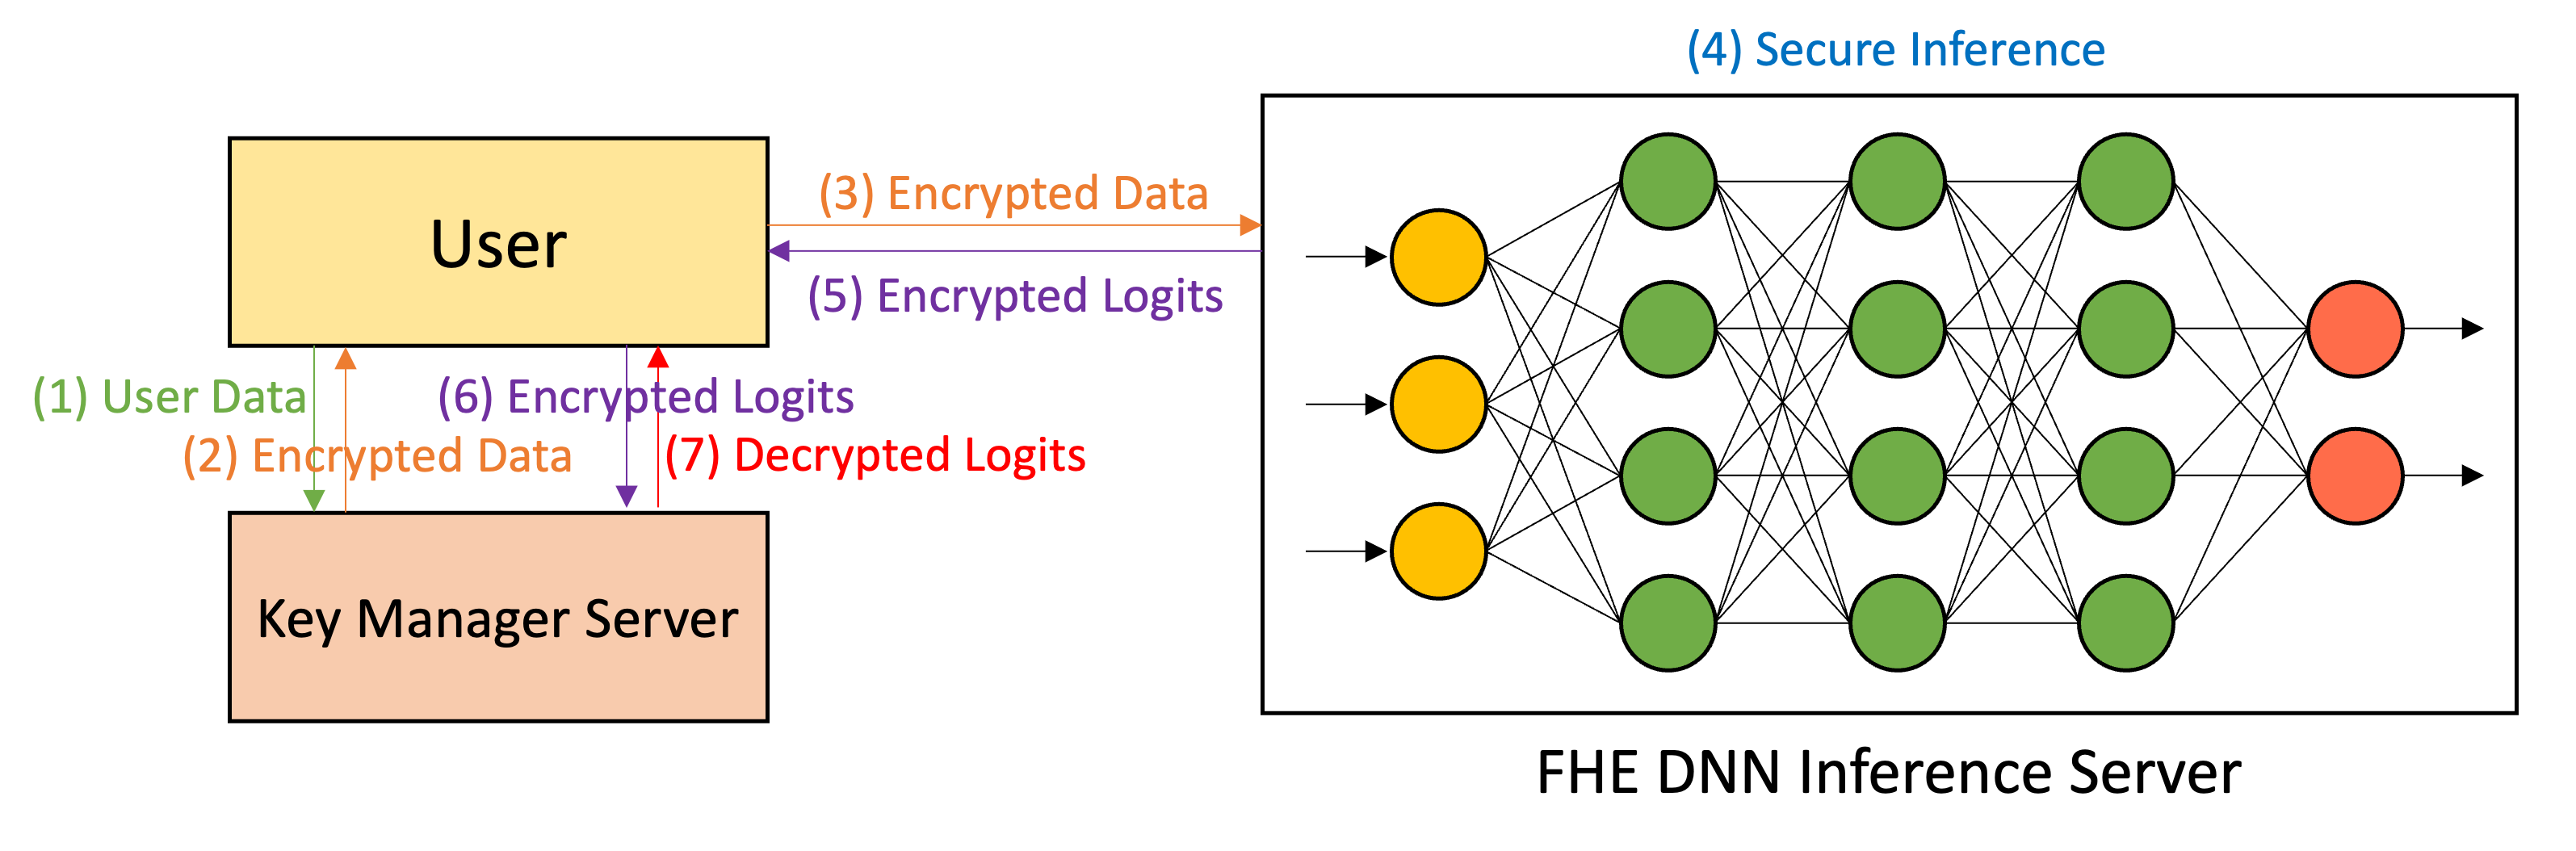
\includegraphics[width=0.9\textwidth]{resource/secure_dnn_inference.png}
  \caption{동형암호 기반 안전한 딥러닝 추론 과정 도식표. 사용자, 키 관리 서버, 딥러닝 추론 서버가 평문 혹은 암호문을 주고받는다. 딥러닝 서버는 암호화된 사용자 데이터의 추론 결과를 계산하지만, 그 과정에서 개인정보를 알아낼 수 없다.}
  \label{fig:secure_dnn_inference}
\end{figure}
우선 사용자, (신뢰할 만한) 키 관리 서버, 그리고 딥러닝 추론 서버로 개체가
구분된다. 사용자의 목표는 자신의 데이터를 암호화된 상태로 외부 네트워크에
전달하여 딥러닝 추론 결과(logits)를 획득하는 것이다. 우선 (1) 사용자는 키 관리
서버에게 자신의 데이터를 전송하여 (2) 암호문을 획득한다. (3) 이를 딥러닝 추론
서버에 전달하고, (4) 동형암호 연산을 사용하여 암호화된 모델 추론 계산 결과를
획득하여 (5) 사용자에게 반환한다. (6) 사용자는 이것을 키 관리 서버에게 보내고,
(7) 복호화한 평문 추론 결과를 가져온다.

이를 통해 딥러닝 추론 서버는 사용자의 데이터와 추론 결과에 대해 아무런 정보도 알
수 없다. 학습된 모델을 네트워크를 사용하여 추론 작업만 수행한 후 사용자에게
결과를 전달해준다.


\chapter{실험 과정}

\section{대상 데이터셋과 모델}

본 실험에서는 하나의 데이터셋과 모델을 가지고 마치 동형암호 상에서 계산하는
것처럼 딥러닝 추론 과정을 시뮬레이션한다. 가장 간단한 MNIST 필기체 데이터셋을
사용했으며, 목표 딥러닝 추론 과정은 분류(classification) 작업이다. 이를 위해
사용했던 분류기 모델은 아래와 같이 구성하였다. (\autoref{fig:network})
\begin{figure}[htbp]
  \centering
  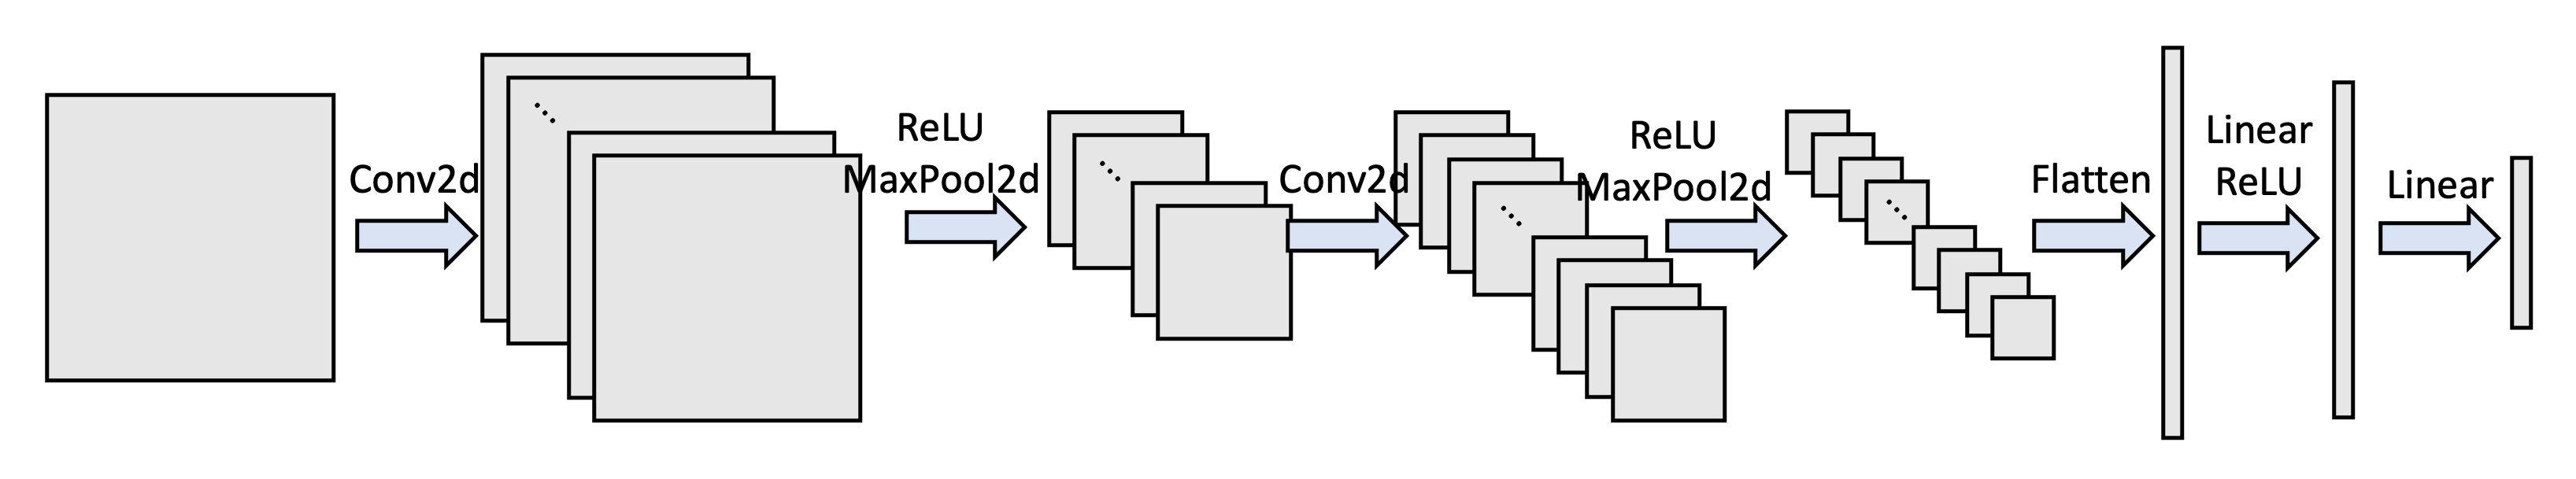
\includegraphics[width=0.9\textwidth]{resource/network.png}
  \caption{MNIST 필기체 숫자 데이터를 분류하기위해 위 뉴럴 네트워크 모델을 사용하였다.}
  \label{fig:network}
\end{figure}

분류기 모델을 구성하는 머신러닝 컴포넌트는 Conv2d, Linear(Matmul), Flatten,
ReLU, 그리고 MaxPool2d가 있다. Conv2d, Linear, 그리고 Flatten은 텐서의 원소에
대한 선형적인 연산자이다. 이들은 마스크(0과 1로 이루어진 텐서)와 곱셈, 그리고
회전($rotate$) 연산을 적절히 사용하면 의미적으로(semantically) 결과가 일치하는
연산 회로를 구성할 수 있다. (\autoref{eqn:matmul})
\begin{figure}[htbp]
  \begin{gather*}
    \frac
      {
        \begin{array}{c}
          \begin{array}{rll}
            \ud{B_1} &:= \ud{B} \: \htimes \: \ud{(1, 0, 0, 1)} &(=\ud{(b_{11}, 0, 0, b_{22})})\\
            \ud{B_2} &:= \hrotate(\ud{B} \: \htimes \: \ud{(0, 0, 1, 0)}, 1)  &(=\ud{(0, b_{21}, 0, 0)})\\
            \ud{B_2} &:= \hrotate(\ud{B} \: \htimes \: \ud{(0, 1, 0, 0)}, -1)  &(=\ud{(0, 0, b_{12}, 0)})\\
            \ud{B^T} &:= \ud{B_1} \:\hplus\: \ud{B_2} \:\hplus\: \ud{B_3} & (=\ud{(b_{11}, b_{21}, b_{12}, b_{22})})\\
            \ud{C_1} &:= \ud{A} \: \htimes \: \ud{B^T} &(=\ud{(a_{11}b_{11}, a_{12}b_{21}, a_{21}b_{12}, a_{22}b_{22})})\\
            \ud{C_2} &:= \hrotate(\ud{A}, 2) \: \htimes \: \ud{B^T} &(=\ud{(a_{21}b_{11}, a_{22}b_{22}, a_{11}b_{12}, a_{12}b_{22})})\\
            \ud{D_1} &:= (\ud{C_1} \: \hplus \: \hrotate(\ud{C_1}, 1)) &(=\ud{(a_{11}b_{11}+a_{12}b_{21},-,a_{21}b_{12}+a_{22}b_{22},-)}) \\
            \ud{D_2} &:= (\ud{C_2} \: \hplus \: \hrotate(\ud{C_2}, 1)) &(=\ud{(a_{21}b_{11}+a_{22}b_{21},-,a_{11}b_{12}+a_{12}b_{22},-)}) \\
          \end{array} \vspace{4px} \\
          \begin{array}{c}
            \ud{X_{11}} := \ud{D_1} \: \htimes \: \ud{(1, 0, 0, 0)},\quad X_{22} := \hrotate(\ud{D_1} \: \htimes \: \ud{(0, 0, 1, 0)}, -1)\\
            \ud{X_{12}} := \hrotate(\ud{D_2} \: \htimes \: \ud{(0, 0, 1, 0)}, 1),\quad X_{21} := \hrotate(\ud{D_1} \: \htimes \: \ud{(1, 0, 0, 0)}, -2) \vspace{4px}\\
            \ud{X} := \ud{X_{11}} \: \hplus \: \ud{X_{12}} \: \hplus \: \ud{X_{21}} \: \hplus \: \ud{X_{22}}
          \end{array}
        \end{array}
      }
      {\ud{AB} = \ud{X}}
  \end{gather*}
  \caption{동형암호 연산만으로 수행하는 $2\times 2$ 행렬 곱셈(Matmul) 수행 예시}
  \label{eqn:matmul}
\end{figure}

하지만 ReLU, MaxPool2d와 같이 텐서 원소의 값에 대한 분기문(conditional
instruction)을 포함하는 컴포넌트는 동형암호에서 계산하기 어렵다. 원소들이
암호화가 되어있기 때문에 그 값이 양수인지 음수인지 판단할 수 없기 때문이다.
그럼에도 불구하고 이러한 요소는 추론 계산 과정에서 비선형성(nonlinearity) 형성을
위해 필수적이므로 근사다항식 등의 방법을 이용하여 해결한다. \cite{compare2019}

\section{분기문과 근사다항식}

실험에서 사용했던 분기문 요소는 ReLU와 MaxPool2d이다. 이들은 모두 결국 절대값
함수를 근사함으로써 구현할 수 있다.
\begin{align*}
  ReLU(x) &= 0.5 \cdot (x + |x|) \\
  MaxPool(x_1, x_2) &= \max(x_1, x_2) = 0.5 \cdot (x_1 + x_2 + |x_1 - x_2|)
\end{align*}
절대값 함수의 근사다항식은 `Chebyshev'와 `Remez'의 근사법으로 건설한다.
\cite{chebapprox} 근사 유효 입력 범위는 $[-1, 1]$로 둔다.

\subsection{Chebyshev 근사다항식}

Chebyshev 방법은 대상 함수와 근사다항식 간의 절대 차이 평균을 최소화한다. (Low
average error) 마치 푸리에 급수 전개와 같이 수직(orthogonal)인 기저(basis)
다항식들을 생성하고, 축 성분의 값을 계수로 두어 합산한 결과를 근사다항식으로
둔다.

우선, 아래와 같은 방식으로 $n+1$개의 다항식 $T_0(x), T_1(x), \dots, T_n(x)$를
생성한다.
\begin{gather*}
  T_0(x) = 1,\quad T_1(x) = x,\quad T_{n+1}(x) = 2x \cdot T_n(x) - T_{n-1}(x)
\end{gather*}
이 다항식은 $n$차원 입력 $(x_k = -\cos(\frac{k \pi}{n}))_{k = 1, 2, \dots, n}$에
대해 계산한 결과가 서로 수직이다.
\begin{align*}
  \sum_{k=1} T_i (x_k) T_j (x_k) = \left\{
    \begin{array}{ll}
      0 & \text{if $i \neq j \leq n$} \\
      n & \text{if $i = j = 0$} \\
      n/2 & \text{if $0 < i = j \leq n$}
    \end{array}
  \right.
\end{align*}
따라서 대상 다항식 $f$를 $f(x) = \sum_{i=0}^n c_i T_i(x)$로 근사하게 된다면 계수
$c_i$는 아래와 같이 계산할 수 있다.
\begin{align*}
  c_i &= \frac{1}{d_i} \sum_{k=1}^n f(x_k) T_i(x_k), \quad
  d_i = \left\{
    \begin{array}{ll}
      n & \text{if $i = 0$} \\
      n/2 & \text{if $i \neq 0$}
    \end{array}
  \right.
\end{align*}

\subsection{Remez 근사다항식}

Remez 방법은 대상 함수와 근사다항식 간의 절대 차이의 최대값을 최소화한다. (Low
maximum error) 아래 정리에 나오는 함수 점들을 획득하기 위해 반복적인(iterative)
알고리즘을 사용한다.

\begin{theorem}[Chebyshev's Equioscillation Theorem]
대상 함수 $f$와 $n$차 이하의 근사다항식 $p$에 대해, 근사 구간 $[a, b]$ 안에서
$||f-p||_\infty$ 값이 최소가 될 필요충분조건은, $a \leq x_1 < x_2 < \cdots <
x_{n+2} \leq b$인 점 $x_1, x_2, \dots, x_{n+2}$이 존재하여 $f(x_i) - p(x_i) =
(-1)^i \cdot ||f-p||_\infty$가 성립하는 것이다.
\end{theorem}

즉, 근사다항식이 함수값보다 커지거나 작아지는 진폭이 일정할 때, 차이의 최대가
최소이다. Remez 알고리즘은 이 성질을 가지는 $x_1, x_2, \dots, x_{n+2}$ 점들을
아래와 같이 반복적으로 찾는다.
\begin{enumerate}
  \item 초기에 점 $x_1, x_2, \dots, x_{n+2}$를 $[-1, 1]$ 구간 안에 증가하는 순서대로 임의로 고른다.
  \item $n+2$개의 미지수 $c_0, c_1, \dots, c_n, E$에 대한 $n+2$개의 일차 연립 방정식을 푼다.
        $$ \left( \sum_{i=0}^n c_i x_k^i \right) + (-1)^k E = f(x_k) $$
  \item $||f(x) - p(x)||$에 대한 극대값(local maximum)들을 찾고 증가하는 순서대로 $x_1, x_2, \dots, x_{n+2}$로 둔 후, 2번 단계로 돌아가 반복한다.
\end{enumerate}

\subsection{다항식 근사 결과}

두 방법에 대해 절대값 함수를 근사한 결과는 아래와 같다.
(\autoref{fig:abs_approx}) Chebyshev 근사 방식은 0 근처의 입력에 대해 뭉뚝한
함수값을 가지지만, 전체적인 오차의 평균은 작다. 또한, 짝수 차수 다항식에 대해
0에 대한 함수값이 다소 위로 올라간 모습을 보인다. Remez 방식은 오차의 최대값이
작으며, 근사함수가 절대값 함수를 오르락 내리락하는 폭의 크기가 일정하다. 차수가
높은 근사식이 더 정확했으며, 이에 직렬적인 곱셈 깊이와 정확도 사이
트레이드오프가 있을 것을 추측해볼 수 있다.
\begin{figure}[htbp]
  \centering
  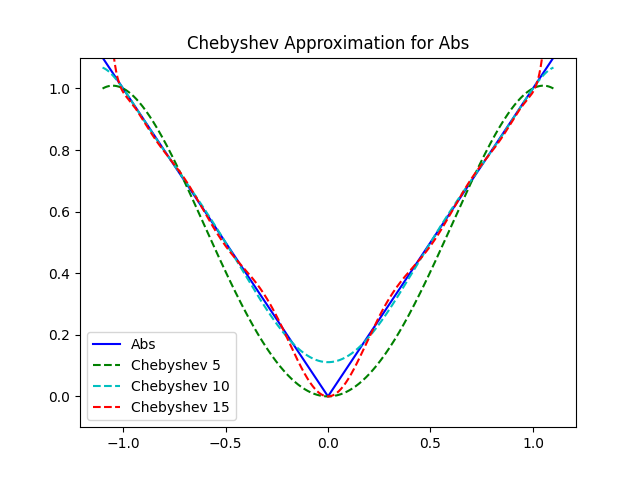
\includegraphics[width=0.45\textwidth]{resource/chebyshev.png}
  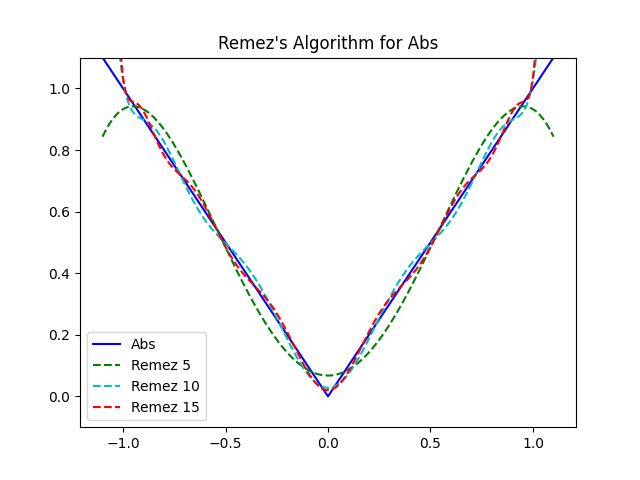
\includegraphics[width=0.45\textwidth]{resource/remez.png}
  \caption{절대값 함수에 대한 Chebyshev 방식의 근사(좌), Remez 방식의 근사(우). Chebyshev 방식은 평균적인 오차의 절대값이 작고, Remez 방식은 오차 절대값의 최대 크기가 작다.}
  \label{fig:abs_approx}
\end{figure}

이를 이용해 ReLU를 계산하고 근사 다항식 유효범위 밖으로 확장한 결과이다.
(\autoref{fig:relu_approx}) 이와 같이 근사 범위인 $[-1, 1]$ 사이에서는 어느 정도
합리적으로 표현이 되었으나, 그 밖의 범위를 조금만 넘어가도 커다란
이상치(outlier)를 발생시킴을 볼 수 있다.
\begin{figure}[htbp]
  \centering
  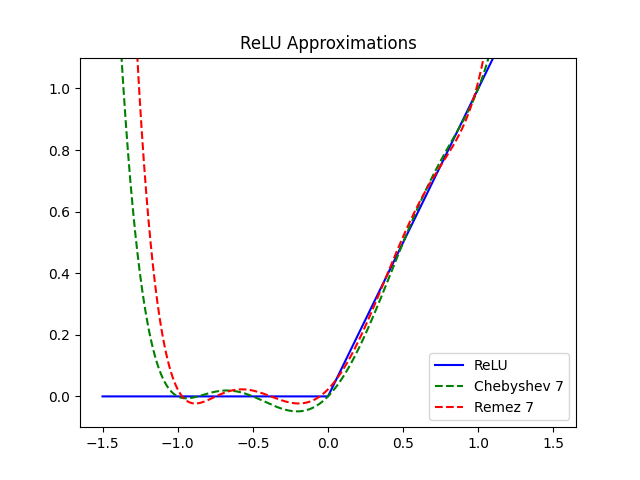
\includegraphics[width=0.6\textwidth]{resource/relu.png}
  \caption{ReLU 함수의 두 근사다항식 결과. 근사 유효 범위인 $[-1, 1]$을 조금만 넘어가도 커다란 이상치(outlier)가 함수값이 나타난다.}
  \label{fig:relu_approx}
\end{figure}

\section{학습 및 추론 시뮬레이션}

우선 `시뮬레이션'이라고 함은 평문 세계에서 PyTorch 라이브러리로 텐서 계산을
하되, 동형암호에서 지원하는 연산(곱셈, 덧셈, 회전)만을 사용하는 것을 의미한다.
즉, 실제로는 평문 텐서에 대해 연산하지만, 마치 암호문에 대해 수행하는 것처럼
취급하면서 목표 함수값을 계산한다.

본 실험에서 동형암호 상에서 일어난다고 가정하는 상황은 오직 `추론' 과정이다.
학습 과정은 이상치를 견디는 배치 정규화, 소프트맥스, 경사 하강법 등 아직
동형암호가 감당하기에 까다로운 부분이 많기 때문이다. 따라서 본 연구에서 딥러닝
모델 학습 단계는 평문 단계에서 이루어진다고 가정한다.

하지만 추론 과정은 동형암호 상에서 이루어진다고 가정하고, 계산의 `효율성'보다는
`정확성'에 더 초점을 두고 실험한다. 따라서 ReLU, MaxPool2d와 같은 분기문 요소를
직접 사용할 수 없고, 오직 근사다항식으로만 계산해야한다. 그러나 Conv2d, Linear,
Flatten과 같은 선형 연산자는 아직은 비효율적이지만 의미적으로 완벽하게 구현하는
방법이 존재하므로, 시뮬레이션에서 그대로 PyTorch API인 \texttt{nn.Conv2d},
\texttt{nn.Linear} 등의 모듈을 사용한다.

\section{고정확도 분류기 학습 과정}

그저 ReLU나 MaxPool2d 구성요소를 근사다항식으로 바꾸는 것만으로는 좋은 정확도를
획득하기 어렵다. 따라서 여러 가지 학습법과 세부 튜닝(fine-tuning) 방법이
필요했다.

\subsection{Activation Decay}

본 실험에서 사용한 근사 다항식은 함수의 입력 범위가 $[-1, 1]$ 사이에 놓이는 것이
중요하다. (\autoref{fig:relu_approx}) 따라서 이 입력 텐서 원소들의 크기(norm)를
손실 함수(loss function)에 activation decay라는 항으로 추가하였다. 손실 함수를
최소화시키는 학습 과정을 거쳤을 때, 근사 다항식의 입력이 가능한 많이 유효 범위
안에 놓이도록 만들었다. 새로 정의된 손실 함수는 다음과 같다.
\begin{align}
  Loss(\vec{\theta}, \vec{x}) = Loss_{orig}(\vec{\theta}, \vec{x})
    + \lambda_{act} \cdot \left( \frac{1}{B} \cdot \sum_{\vec u \in \text{inputs of approx.}} ||\vec u||_p \right)
  \label{eqn:act_decay}
\end{align}
여기서 $\lambda_{act}$ 값을 activation decay coefficient라고 하고, 크기를
조절해가며 결과를 측정했다.

\subsection{LeakyReLU}

LeakyReLU란 음의 입력에 대해서도 미약한 기울기를 두는 ReLU 함수의 대체품이다.
($u \in (0, 1)$, 보통 $u$는 $0.1$의 값을 가진다.)
\begin{gather*}
  LeakyReLU(x) = \left\{
    \begin{array}{ll}
      x & \text{if $x \geq 0$} \\
      ux & \text{if $x < 0$}
    \end{array}
  \right.
  \quad = \frac{1+u}{2} \cdot \left( x + \frac{1-u}{1+u} \cdot |x| \right)
\end{gather*}

ReLU 함수의 근사 다항식은 음의 입력에 대한 함수값이 들쑥날쑥하여 완벽한
상수함수가 아니다. (\autoref{fig:relu_approx}) 그러나 LeakyReLU의 근사식은 음의
입력에 대해서도 함수값이 감소하는 경향성이 지켜지므로, 근사의 오차가 줄어들 것으로
기대하였다.

\subsection{최적 학습 파이프라인}

여러 실험을 반복하며 얻을 수 있었던 최적의 실험 설정은 아래와 같았다.
\begin{enumerate}
  \item (Big-step) 모델을 작은 activation decay($\lambda_{act, 1} = 10^{-4}$)로 오랫동안(20 에포크) 학습한다.
  \item (Large decay) 모델은 큰 activation decay($\lambda_{act, 2} = 10^{-2}$)로 조금 더(10 에포크) 학습한다.
  \item (Fine-tune) 모델에서 분기문 요소를 근사다항식으로 대체한 후, 큰 activation decay($\lambda_{act, 3} = 10^{-2}$)로 조금 더(10 에포크) 학습한다.
\end{enumerate}
공통적으로 multi-step learning rate scheduler를 사용하였다. 초기 learning rate를
$\alpha$라고 했을 때, $50\%$의 에포크 진행 후 $0.1 \cdot \alpha$, $75\%$ 진행 후
$0.01 \cdot \alpha$로 학습하였다. 1번 big-step 단계에서는 $\alpha = 0.1$로, 2,
3번 단계에서는 $\alpha = 0.001$로 초기값을 두고 학습했다.

여러 실험 결과를 획득하고 비교하기 위해 조작변인으로써 아래와 요인을 두었다.
\begin{itemize}
  \item 근사다항식의 방법(Chebyshev와 Remez)과 최고차항
  \item ReLU 대신 LeakyReLU 사용
  \item Activation decay로써 $L1$ 혹은 $L2$-norm 사용
  \item 마지막 fine-tune 단계에서 activation decay 계수 크기 ($\lambda_{act, 3}$)
\end{itemize}

실험과 관련된 모든 코드는
\url{https://github.com/lego0901/fhe_secure_inference_simulation} 깃헙 링크에서
접근할 수 있다.


\chapter{실험 결과}

\section{조작변인에 따른 실험 결과 비교}

첫 번째 결과는 LeakyReLU와 그냥 ReLU의 정확도 비교 실험이다.
(\autoref{fig:result_leaky}) 모두 같은 1(Big-step), 2(Large decay),
3(Fine-tune)번 과정을 거쳤으며, activation decay로 $L1$-norm을 사용한 결과이다.
$\lambda_{act,3}=10^{-2}$인 기본값을 사용했을 때, ReLU를 사용하는 것이
LeakyReLU를 사용하는 것보다 훨씬 안정적이고 높은 정확도를 가져왔다.
\begin{figure}[htbp]
  \centering
  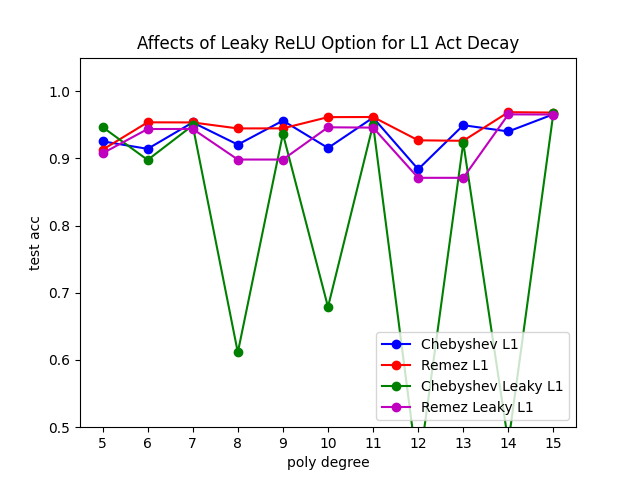
\includegraphics[width=0.5\textwidth]{resource/leaky.png}
  \caption{$L1$-norm의 activation decay에서 ReLU와 LeakyReLU의 정확도 비교. ReLU를 사용하는 것이 더 안정적이고 높은 정확도를 가져왔다.}
  \label{fig:result_leaky}
\end{figure}

그 다음은 $L2$-norm으로 activation decay를 구성한 결과이다.
(\autoref{fig:result_leaky_l2}) 이번에는 근사다항식의 차수에 따라 결과가
불안정했지만, LeakyReLU를 사용하는 것이 조금 더 정확도가 좋았다. 따라서
$L1$-norm은 ReLU와, $L2$-norm은 LeakyReLU와 조합했을 때 정확하다는 것을 알 수
있었다. 또한, 의외로 낮은 차수의 근사식에서 더 좋은 결과가 나타났다.
\begin{figure}[htbp]
  \centering
  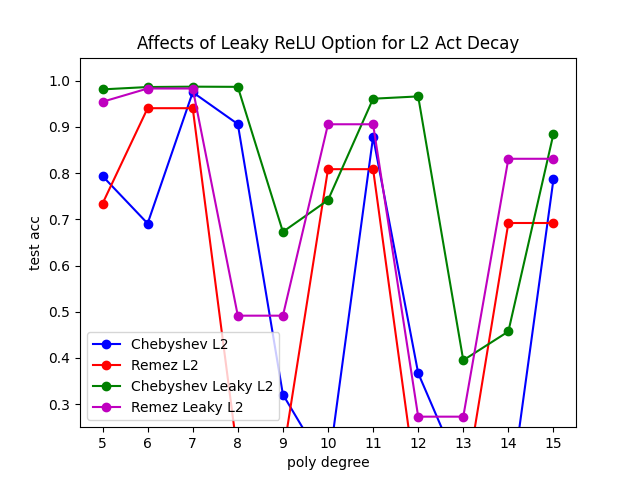
\includegraphics[width=0.5\textwidth]{resource/leaky_l2.png}
  \caption{$L2$-norm의 activation decay에서 ReLU와 LeakyReLU의 정확도 비교. $L1$-norm은 ReLU와, $L2$-norm은 LeakyReLU와 조합했을 때 효과적이었다. 또한, 낮은 차수 다항식이 좋았다.}
  \label{fig:result_leaky_l2}
\end{figure}

좋은 조합이었던 $L1$-norm과 ReLU, 그리고 $L2$-norm과 LeakyReLU 결과를 한 곳에
모았다. (\autoref{fig:result_norm}) 전자의 조합은 차수에 상관없이 두루 높은
정확도 결과를 가져왔다. 후자 조합은 안정성은 떨어졌으나, 최고 정확도에서 가장
뛰어난 결과를 가져왔다.
\begin{figure}[htbp]
  \centering
  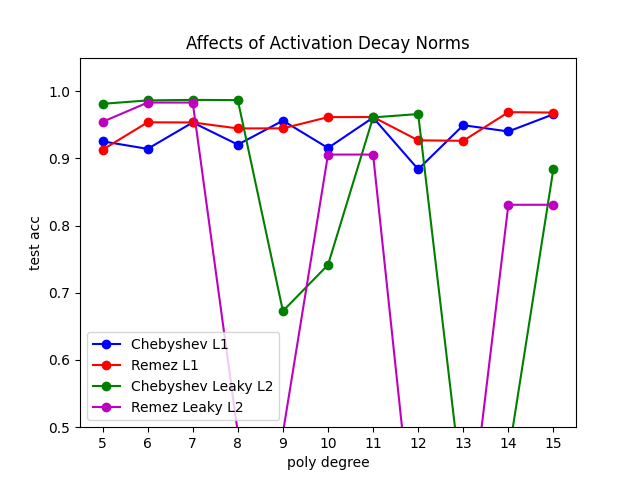
\includegraphics[width=0.5\textwidth]{resource/norm.png}
  \caption{$L1$+ReLU와 $L2$+LeakyReLU 조합의 정확도 비교. 전자 조합은 안정성이, 후자는 최고 정확도가 좋았다.}
  \label{fig:result_norm}
\end{figure}

마지막 3단계(Fine-tuine)에서 activation decay 계수 $\lambda_{act, 3}$를
조정해가며 실험 결과를 비교했다. (\autoref{fig:result_decay}) $\lambda_{act,
3}$의 값이 컸을 때 ($10^{-2}$) 조금 더 안정적인 결과를 가져왔다. 하지만 낮은
차수 다항식에서 더 작은 계수가 ($10^{-3}$) 최고 정확도 면에서는 더 우수한 값을
가져왔다.
\begin{figure}[htbp]
  \centering
  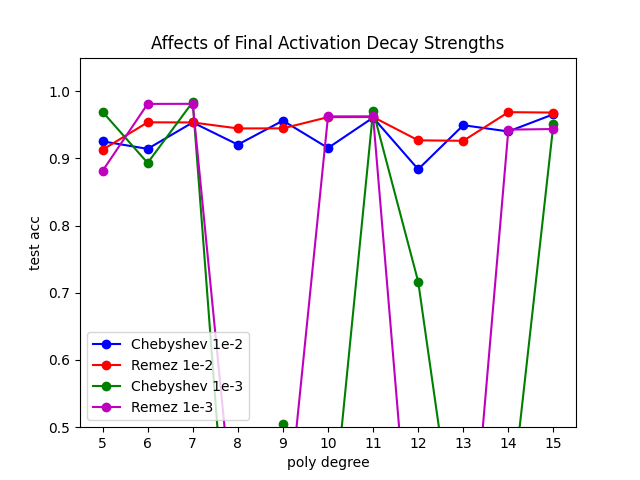
\includegraphics[width=0.5\textwidth]{resource/decay.png}
  \caption{$L1$-norm activation decay 계수에 따른 정확도 비교. $\lambda_{act,3}$이 큰 값일 때 안정적이다. 다만, 낮은 차수 근사식은 작은 값일 때 정확도가 높다.}
  \label{fig:result_decay}
\end{figure}

이번에는 2(Large decay), 3(Fine-tune) 단계 없이, 학습과정에 사용되었던 분기문
컴포넌트를 추론 과정에서 근사다항식으로 교체하기만 한다면 정확도에 어떤 영향을
미치는지 실험해보았다. (\autoref{fig:result_finetune}) 모든 상황에 대해서 세부
튜닝을 한 것이 정확도가 좋았으며, 이에 근사다항식으로 교체한 후 추가 학습 작업이
필수적임을 시사하는 결과라고 볼 수 있다.
\begin{figure}[htbp]
  \centering
  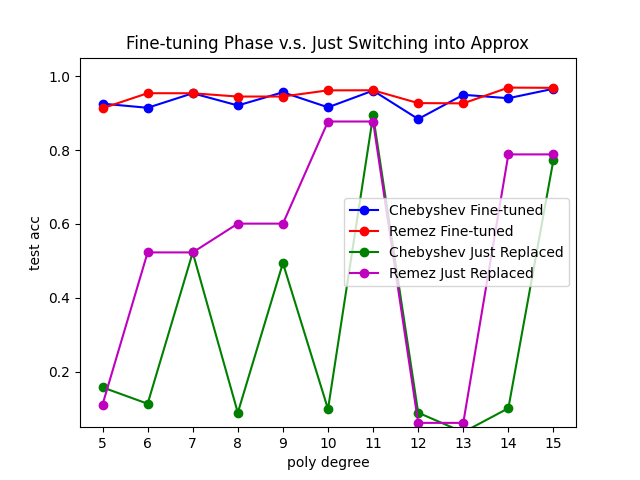
\includegraphics[width=0.5\textwidth]{resource/finetune.png}
  \caption{2, 3단계의 세부 튜닝 과정없이 단순히 분기문 컴포넌트를 근사다항식으로 교체한 결과 비교. 세부 튜닝한 것이 정확도나 안정성 면에서 모두 우수했다.}
  \label{fig:result_finetune}
\end{figure}

2단계 (Large decay)의 역할에 대해 실험해보았다. 만약 적절히 큰 activation decay
계수 $\lambda_{act, 2}$를 사용하지 않고 학습한 후 3단계 (Fine-tune)만 진행하면
어떤 결과가 나타나는지 확인해보았다. (\autoref{fig:result_act}) 놀랍게도 짝수
차수의 Chebyshev 근사 방법에서 큰 폭의 정확도 하락이 나타났다.
\begin{figure}[htbp]
  \centering
  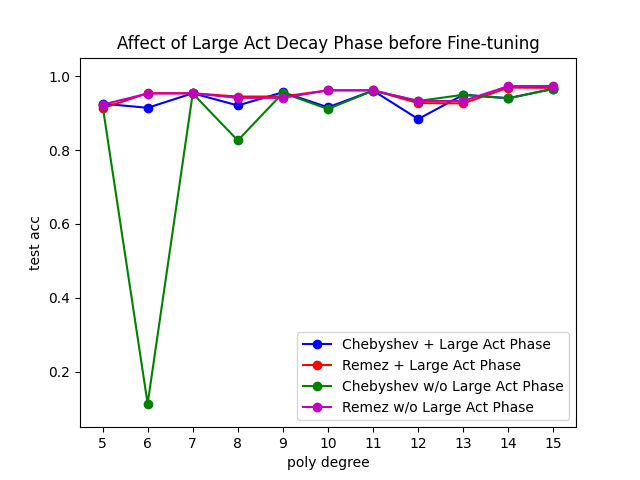
\includegraphics[width=0.5\textwidth]{resource/act.png}
  \caption{2단계 (Large decay) 과정없이 단순히 3단계 (Fine-tune)만 시킨 결과 비교. 2단계 단계를 거친 것이 안정적이다.}
  \label{fig:result_act}
\end{figure}

정확도 그래프만 살펴보는 것이 아니라, 근사다항식의 입력으로 들어오는 텐서
원소들의 절대값 크기 분포를 조사해보았다. 이 입력은 $[-1, 1]$ 범위 내에서
유효하기 때문에 가능한 크기가 작을 수록 더 좋은 정확도를 보일 가능성이 있다.
3단계 Fine-tune의 여부에 따라 분포가 어떻게 달라지는지 시각화했다.
(\autoref{fig:result_finetune_profile}) 확실히 세부 튜닝을 거친 모델이 그렇지
않은 것보다 훨씬 크기가 적은 값들로 분포가 몰렸음을 확인할 수 있다.
\begin{figure}[htbp]
  \centering
  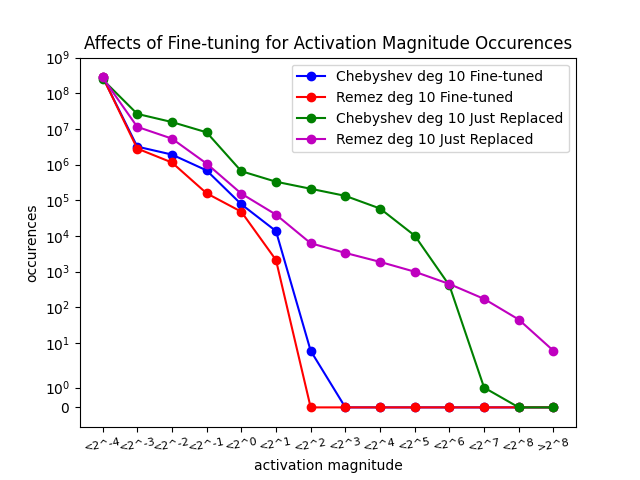
\includegraphics[width=0.5\textwidth]{resource/finetune_profile.png}
  \caption{3단계 (Fine-tune)의 실행 여부에 따른 근사다항식 입력 절대값 크기 분포 비교. 세부 튜닝을 거쳤을 때 입력의 분포가 작은 값으로 몰린다.}
  \label{fig:result_finetune_profile}
\end{figure}

\newpage
\section{최고 성능 실행 환경 정리}

결과적으로 가장 높은 성능을 얻었던 실행 환경을 정리하면 \autoref{tab:top_acc}와
같다.
\begin{table}[htbp]
  \center
  \begin{tabular}{|c|c|c|c|} \hline
    Approximates & Act Decay & ReLU Layer & Accuracies \\ \hline
    \alert{Chebyshev 7} & \alert{L2, $\lambda_{act,3}=10^{-2}$} & \alert{LeakyReLU} & \alert{98.71} \\
    Chebyshev 8 & L2, $\lambda_{act,3}=10^{-2}$ & LeakyReLU & 98.67 \\
    Chebyshev 6 & L2, $\lambda_{act,3}=10^{-2}$ & LeakyReLU & 98.63 \\
    \alert{Chebyshev 7} & \alert{L1, $\lambda_{act,3}=10^{-3}$} & \alert{ReLU} & \alert{98.39} \\
    \alert{Remez 7} & \alert{L2, $\lambda_{act,3}=10^{-2}$} & \alert{LeakyReLU} & \alert{98.31} \\
    Remez 6 & L2, $\lambda_{act,3}=10^{-2}$ & LeakyReLU & 98.31 \\
    Remez 10 & L2, $\lambda_{act,3}=10^{-2}$ & LeakyReLU & 98.21 \\
    Remez 11 & L2, $\lambda_{act,3}=10^{-2}$ & LeakyReLU & 98.21 \\
    Chebyshev 5 & L2, $\lambda_{act,3}=10^{-2}$ & LeakyReLU & 98.12 \\
    \alert{Remez 5} & \alert{L1, $\lambda_{act,3}=10^{-3}$} & \alert{ReLU} & \alert{98.12} \\
    Remez 6 & L1, $\lambda_{act,3}=10^{-3}$ & ReLU & 98.11 \\
    \hline
  \end{tabular}
  \caption{가장 높은 정확도를 가지는 실행 환경 조합 정리}
  \label{tab:top_acc}
\end{table}
낮은 차수의 근사다항식이 더 좋은 결과를 내는 경우가 많았다. $L2$-norm에서는
$\lambda_{act,3}=10^{-2}$의 큰 값으로 LeakyReLU를 쓰는 경우에 효과적이었으며,
$L1$-norm에서는 반대로  $\lambda_{act,3}=10^{-3}$의 작은 값으로 ReLU를 쓰는 것이
더 좋았다.

표에서 대표적인 실행 환경에 대해 근사다항식 입력 텐서 절대값 크기 분포를
시각화하면 \autoref{fig:result_tops_profile}와 같다. $L2$를 사용하는 것은
입력값의 분포를 더 분산시켰다. y축 성분의 단위가 로그 스케일인 것을 감안하면, 더
입력 유효 범위 안으로 잘 모았던 것은 $L2$-norm이었던 것으로 판단된다.
\begin{figure}[htbp]
  \centering
  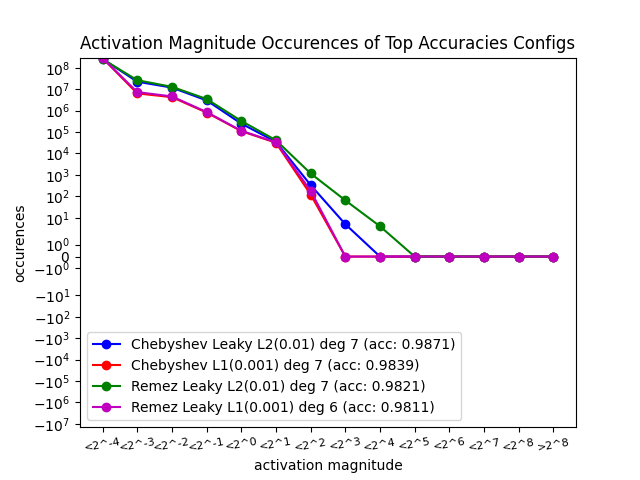
\includegraphics[width=0.5\textwidth]{resource/tops_profile.png}
  \caption{가장 높은 정확도를 가지는 실행 환경의 근사다항식 입력 절대값 크기 분포 비교. 모두 우수한 분포를 보여줬으나, $L2$-norm이 조금 더 유효한 범위 안으로 숫자를 잘 모아주었다.}
  \label{fig:result_tops_profile}
\end{figure}


\chapter{결론}

\section{실험 결론}

동형암호 기반 딥러닝 추론 시스템을 시뮬레이션하기 위해 분기문 컴포넌트를 절대값
함수의 근사다항식으로 교체했다. Chebyshev와 Remez의 알고리즘에서 최고차수를
달리해가며 사용했다. 학습 과정에서 근사다항식의 입력이 가능한 유효한 범위인
$[-1, 1]$ 내에 놓이게 만들기 위해 activation decay라는 개념을 도입했고, 음의
입력에 대한 오차를 줄이기 위해 LeakyReLU를 ReLU 대신 사용하기도 했다. 모델의
정확도를 유지하기 위해 1단계 big-step, 2단계 large-decay, 3단계 fine-tune 과정을
거쳤다.

결과적으로 1, 2, 3 모든 단계가 입력의 분포를 더 안정적으로 바꾸는 등 유의미한
성능 향상을 일구어냈음을 밝혀냈다. [$L1$-norm과 낮은 fine-tune 단계의 activation
decay $\lambda_{act,3}=10^{-3}$와 ReLU]의 조합, 혹은 [$L2$-norm과 높은 fine-tune
단계의 activation decay $\lambda_{act,3}=10^{-2}$와 LeakyReLU]의 조합이 높은
성능을 얻었다. 원래는 고차 근사 다항식이 더 좋은 정확도를 획득하는 대신 noise
level에서 손해를 보는 트레이드오프 관계 결과를 예상했으나, 반대로 낮은 차수의
식들이 더 안정적이고 높은 정확도를 보였다. 이로부터 분기문 요소를 범위 내에서
정확히 계산하는 것보다, 이상치(outlier) 값을 덜 극단적으로 만드는 것이 더
중요했음을 결론지을 수 있었다.

\section{추후과제}

이번 연구는 딥러닝 추론 과정을 `시뮬레이션'한 것에 그친다는 한계가 있었다.
실제로 동형암호 시스템 상에서 구현하기 위해서는 수많은 선행 연구가 요구된다.
의미적으로 결과가 일치하는 연산 회로를 구성할 수 있다고 본 연구에서 간단히
넘어간 Conv2d, Matmul 등도 실제로 동형암호의 연산만으로 수행하는 구체적이고
효율적인 방법이 제시되어야 한다. 이는 \autoref{eqn:matmul}에서 살펴보았듯 그리
간단하지 않다. 또한 noise level을 트래킹하여 적절한 시기에
재부팅(bootstrapping)을 삽입해주어야하며, 그 횟수를 줄이는 최적화 연구도
필요하다. 이렇듯 시뮬레이션을 벗어나 실제 구현을 하기 위해서는 추후 수많은
기술과 논의가 필요할 것이다.


\printbibliography[title=참고문헌]


\chapter*{Abstract}
\begin{quote}
A secure deep neural network (DNN) inference system based on homomorphic
encryption (HE) is a rising topic investigated by academia and industry. It is
because it attains perfect privacy while performing the network inference. Many
recent studies are actively decomposing ML components into HE building block
operations or optimizing them at high and low levels. However, after these
processes, it should also be discussed to maintain performance (accuracy) by
training and fine-tuning the model to suit the characteristics of HE. This study
aims to simulate the DNN inference process in the HE system and find a model
training method that preserves accuracy as much as possible. Simulations
experimentally discover model training methodologies that replace conditional
instructions which cannot be computed from a ciphertext with an approximate
polynomial, minimizing the accuracy drop. The usability of a secure DNN system
that inferences from encrypted user data without decryption shall be
reconsidered afterward.
\end{quote}

\begin{center}
  \textbf{Keywords: Homomorphic Encryption, Secure DNN Inference,\\
  Simulation, Approximate Polynomial, Model Training}
\end{center}


\end{document}